\def \kaflanr {14}
\lecture[\kaflanr]{\kaflanr. Breytuskipti}{lecture-text}
\date{18.~febrúar 2015}
\newcounter{mycount}
\refstepcounter{mycount}

\begin{document}

\subsection{}
	\maketitle





\subsection{} 

\subsubsection{Upprifjun \kaflanr.\arabic{mycount}}\stepcounter{mycount}
 Látum $P=(x,y)\neq \ov$ vera punkt í plani.  {\em
  Pólhnit} $P$ er talnapar $[r,\theta]$ þannig að $r$ er fjarlægð $P$
frá 
$O=(0,0)$ og $\theta$ er hornið á milli striksins $\overline{OP}$ og
  $x$-ássins.  (Hornið er mælt þannig að rangsælis stefna telst
  jákvæð, og leggja má við $\theta$ heil margfeldi af $2\pi$.) 




\subsection{} 

\subsubsection{Skilgreining \kaflanr.\arabic{mycount}}\stepcounter{mycount}
 {\em Pólhnitarétthyrningur} í $xy$-planinu
er svæði sem afmarkast af tveimur hringbogum $x^2+y^2=a^2$ og
$x^2+y^2=b^2$ og tveimur hálflínum sem byrja í $(0,0)$ og mynda hornin
$\alpha$ og $\beta$ við $x$-ásinn (Hornin eru mæld þannig að rangsælis
stefna telst jákvæð.) 
\begin {figure}[h!]
 \centering
            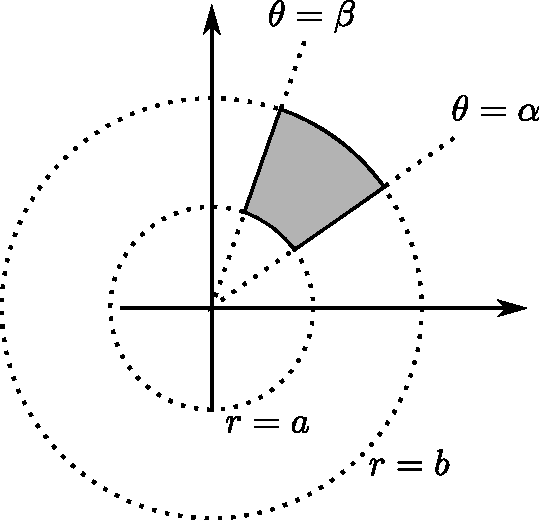
\includegraphics[width=0.35\linewidth]{polarrett}
\end {figure}
Gerum ráð fyrir að $0\leq a\leq b$ og að $0\leq\beta-\alpha\leq
2\pi$.  Þá má lýsa pólhnitarétthyrningnum með því  að nota pólhnit
þannig að 
$$D=\{[r,\theta]\mid 0\leq a\leq r\leq b, \alpha\leq \theta\leq\beta\}.$$
 




\subsection{} 

\subsubsection{Setning \kaflanr.\arabic{mycount}}\stepcounter{mycount}
Ef $f$ er fall sem er heildanlegt yfir 
pólhnitarétthyrning
$D=\{[r,\theta]\mid 0\leq a\leq r\leq b, \alpha\leq \theta\leq\beta\}$
þá er 
$$\tvint_D f(x,y)\,dA=\int_\alpha^\beta\!\!\!\int_{a}^{b}
f(r\cos\theta,r\sin\theta)\,r\,dr\, d\theta.$$

\begin {figure}[h!]
 \centering
            
\includegraphics[width=0.85\linewidth]{polarelement}
\end {figure}


\subsection{} 

\subsubsection{Upprifjun \kaflanr.\arabic{mycount}}\stepcounter{mycount}
Látum $f$ vera fall skilgreint á bili 
$[\alpha,\beta]$.  Jafnan $r=f(\theta)$ lýsir mengi allra punkta í
planinu sem hafa pólhnit á forminu $[f(\theta),\theta]$ þar sem
$\alpha\leq\theta\leq\beta$.  Þetta mengi kallast {\em pólhnitagraf}
fallsins $f$. 






\subsection{} 

\subsubsection{Setning \kaflanr.\arabic{mycount}}\stepcounter{mycount}
Látum $D$ vera svæði i $xy$-plani sem
afmarkast ef pólhnitalínum $\theta=\alpha$ og $\theta=\beta$ og
tveimur pólhnitagröfum $r=a(\theta)$ og $r=b(\theta)$.  Gerum ráð
fyrir að $0\leq a(\theta)\leq
r\leq b(\theta)$ og $0\leq \beta-\alpha\leq 2\pi$.
Ef $f$ er heildanlegt fall yfir $D$
þá er 
$$\tvint f(x,y)\,dA=\int_\alpha^\beta\!\!\!\int_{a(\theta)}^{b(\theta)}
f(r\cos\theta,r\sin\theta)\,r\,dr\, d\theta.$$


\begin {figure}[h!]
 \centering
            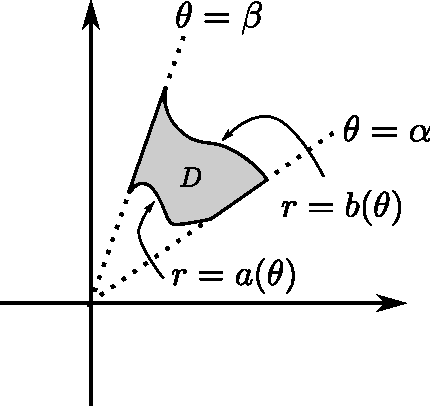
\includegraphics[width=0.35\linewidth]{polarsvaedi}
\end {figure}



\subsection{} 

\subsubsection{Regla \kaflanr.\arabic{mycount}}\stepcounter{mycount}
Hugsum okkur að $f(x,y)$ sé fall og hægt sé að rita
$f(x,y)=g(x)h(y)$.  Látum $R=[a,b]\times [c,d]$.  Þá er 
\begin{align*}
\tvint_R f(x,y)\,dA&=\int_a^b\!\!\!\int_{c}^{d}g(x)h(y)\,dy\, dx\\
&=\bigg(\int_a^b g(x)\,dx\bigg)\bigg(\int_c^d h(y)\,dy\bigg).
\end{align*}





\subsection{} 

\subsubsection{Setning \kaflanr.\arabic{mycount} (Almenn breytuskiptaregla fyrir tvöföld heildi)}\stepcounter{mycount}

Látum $x=x(u,v)$, $y=y(u,v)$ vera gagntæka vörpun milli svæðis $S$ í
$uv$-plani og svæðis $D$ í $xy$-plani.  Gerum ráð fyrir að föllin  
$x(u,v)$, $y(u,v)$ hafi samfelldar fyrsta stigs hlutafleiður á $S$.  Ef
$f$ er heildanlegt fall yfir $D$, þá er fallið $g(u,v)=f(x(u,v), y(u,v))$
heildanlegt yfir $S$ og 
$$\tvint_D f(x,y)\,dx\,dy=\tvint_S g(u,v)
\bigg|\frac{\partial(x,y)}{\partial(u,v)}\bigg|\,du\,dv.$$

\begin {figure}[h!]
 \centering
            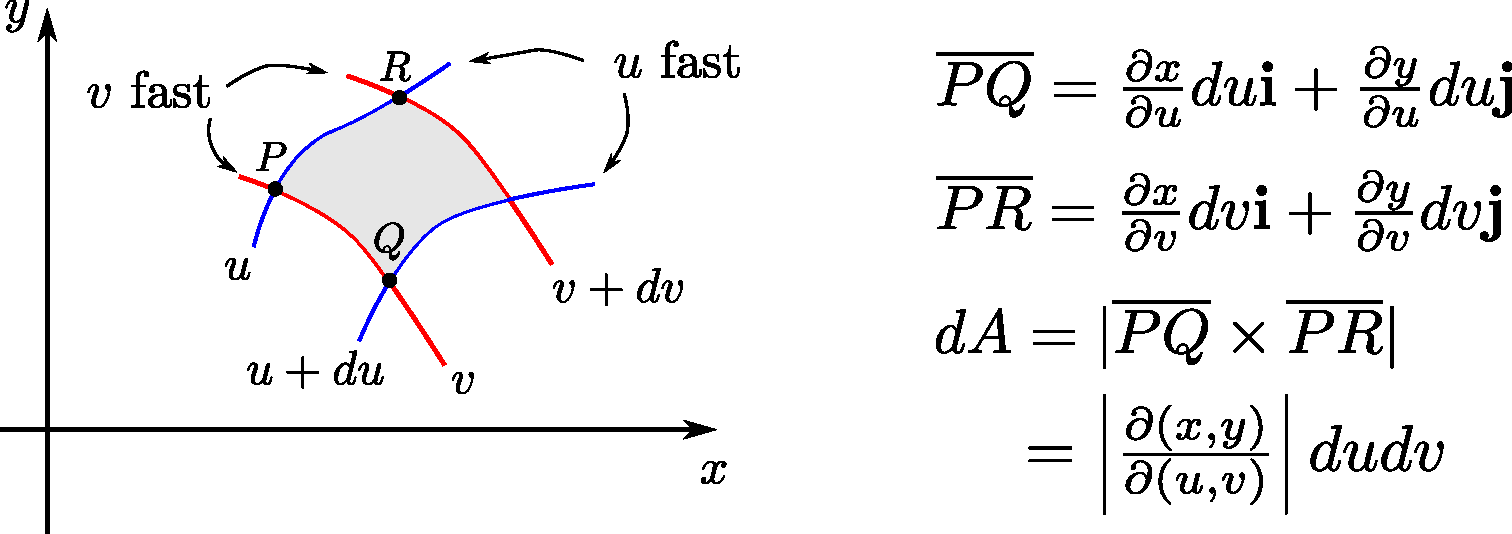
\includegraphics[width=0.85\linewidth]{changevar}
\end {figure}




\end{document}